% !TeX encoding = UTF-8
\documentclass[conference]{IEEEtran}

% ── Paketler ──
\usepackage[utf8]{inputenc}
\usepackage[T1]{fontenc}
\usepackage[turkish]{babel}
\usepackage{amsmath,amssymb,amsfonts}
\usepackage{graphicx}
\usepackage{textcomp}
\usepackage{xcolor}
\usepackage{hyperref}
\usepackage{listings}
\usepackage{booktabs}
\usepackage{float}
\usepackage{cite}
\usepackage{url}
\usepackage{array}
\usepackage{multirow}
\usepackage{enumitem}

% ── Listings ayarları ──
\lstset{
  basicstyle=\ttfamily\small,
  breaklines=true,
  frame=single,
  language=Python,
  showstringspaces=false,
  tabsize=2,
  captionpos=b,
  numbers=left,
  numberstyle=\tiny\color{gray},
  keywordstyle=\color{blue},
  stringstyle=\color{red},
  commentstyle=\color{green!60!black},
}

% ── Hyperref ayarları ──
\hypersetup{
  colorlinks=true,
  linkcolor=blue,
  citecolor=blue,
  urlcolor=blue
}

\begin{document}

\title{Yazılım labrotuvarı 1.Proje}

\author{
\IEEEauthorblockN{Mohamed Younes}
\IEEEauthorblockA{
İzmit/Kocaeli \\
230202016@kocaeli.edu.tr
}
\and
\IEEEauthorblockN{Merve Sevim}
\IEEEauthorblockA{
İzmit/Kocaeli \\
230202035@kocaeli.edu.tr
}
}

\maketitle

% ──────────────────────────────────────────────
\textbf{Anahtar Kelimeler:} 
Web kazıma, doğal dil işleme, haber sınıflandırma, konum çıkarımı, coğrafi kodlama, Google Maps, MongoDB, FastAPI, Next.js

% ──────────────────────────────────────────────
\section{Giriş}
\label{sec:giris}

Bu çalışmada, Kocaeli iline ait yerel haber kaynaklarından otomatik veri toplama, doğal dil işleme teknikleri ile içerik analizi ve Google Maps üzerinde dinamik görselleştirme sağlayan kapsamlı bir haber takip sistemi sunulmaktadır. Geliştirilen sistem; beş farklı yerel haber sitesinden web kazıma (web scraping) yöntemiyle haberleri toplamakta, metin ön işleme ve temizleme adımlarından geçirmekte, anahtar kelime tabanlı sınıflandırma ile haber türünü belirlemekte, metin içerisinden konum bilgisi çıkararak coğrafi koordinatlara dönüştürmekte ve gömme (embedding) tabanlı benzerlik analizi ile tekrarlı haberleri tespit etmektedir. Sistem, Python FastAPI ile geliştirilen asenkron bir arka uç (backend) ve Next.js ile oluşturulan modern bir ön yüz (frontend) mimarisinden oluşmakta olup MongoDB veritabanı kullanılmaktadır. Deneysel sonuçlar, sistemin yüksek doğrulukla haberleri sınıflandırabildiğini, konum bilgisini çıkarabildiğini ve tekrarlı haberleri başarılı bir şekilde filtreleyebildiğini göstermektedir.

Günümüz şehir yaşamında trafik kazaları, elektrik kesintileri, hava durumu uyarıları, toplumsal etkinlikler ve çeşitli acil durumlar gibi birçok dinamik olay sürekli olarak meydana gelmektedir. Bu olaylar genellikle haber siteleri, belediye duyuruları ve dijital medya platformları aracılığıyla kamuoyuna duyurulmaktadır. Ancak bu bilgilerin farklı kaynaklarda dağınık halde bulunması, kullanıcıların güncel olaylara bütüncül ve hızlı bir şekilde erişimini zorlaştırmaktadır \cite{liu2019}.

Bu çalışma kapsamında, Kocaeli iline ait beş farklı yerel haber sitesinden haberlerin otomatik olarak toplanması, işlenmesi ve Google Maps üzerinde interaktif bir harita aracılığıyla görselleştirilmesi sağlayan bir sistem geliştirilmiştir. Geliştirilen sistem; web kazıma (web scraping) teknikleri ile haber verisi toplamakta, doğal dil işleme (NLP) yöntemleri ile metinleri temizlemekte ve sınıflandırmakta, konum çıkarımı ve coğrafi kodlama (geocoding) işlemleri ile haberlerin harita üzerinde gösterimini sağlamakta ve embedding tabanlı benzerlik analizi ile tekrarlı haberleri filtrelemektedir.

Sistemin temel katkıları şu şekilde özetlenebilir:

\begin{itemize}[leftmargin=*]
    \item Beş farklı Kocaeli yerel haber kaynağından eş zamanlı ve asenkron veri toplama altyapısı,
    \item Kapsamlı metin ön işleme hattı ile reklam, şablon ve gereksiz içerik temizliği,
    \item Anahtar kelime tabanlı otomatik haber sınıflandırma mekanizması,
    \item Kocaeli ilçe, mahalle ve önemli yer adlarına dayalı konum çıkarım algoritması,
    \item Google Geocoding API entegrasyonu ile MongoDB tabanlı önbellek (cache) mekanizması,
    \item Çok dilli cümle gömme (sentence embedding) modeli ile \%90 eşik değerinde tekrar tespit sistemi,
    \item RESTful API tabanlı modüler mimari ve sunucusuz (serverless) dağıtım desteği.
\end{itemize}

% ──────────────────────────────────────────────
\section{İlgili Çalışmalar}
\label{sec:ilgili}

Web kazıma ve haber analizi alanında çeşitli çalışmalar gerçekleştirilmiştir. Mitchell \cite{mitchell2018}, Python ekosistemindeki web kazıma tekniklerini kapsamlı bir şekilde ele almış ve BeautifulSoup kütüphanesinin HTML ayrıştırma üzerindeki etkinliğini göstermiştir. Jurafsky ve Martin \cite{jurafsky2024}, doğal dil işleme tekniklerinin metin sınıflandırma ve bilgi çıkarımı üzerindeki uygulamalarını incelemiş olup metin ön işleme adımlarının model başarımına olan etkisini vurgulamışlardır.

Haber görselleştirme alanında Gao vd. \cite{gao2020}, coğrafi bilgi sistemleri (GIS) ile haber verilerinin entegrasyonunu araştırmış ve harita tabanlı görselleştirmenin kullanıcı deneyimini önemli ölçüde iyileştirdiğini raporlamışlardır. Reimers ve Gurevych \cite{reimers2019}, çok dilli cümle gömme modellerinin metin benzerlik analizi üzerindeki başarımını değerlendirmiş ve \texttt{paraphrase-multilingual-MiniLM-L12-v2} modelinin düşük kaynak tüketen ancak yüksek performans gösteren bir alternatif olduğunu belirtmişlerdir.

MongoDB gibi NoSQL veritabanlarının esnek şema yapısı ve ölçeklenebilirlik avantajları, özellikle yarı yapılandırılmış veri kümeleri için uygun bir seçenek olarak değerlendirilmektedir \cite{mongodb2024}. FastAPI çerçevesi ise asenkron programlama desteği ve otomatik API dokümantasyonu özellikleri ile modern web uygulamaları için tercih edilen bir araç haline gelmiştir \cite{fastapi2024}.

% ──────────────────────────────────────────────
\section{Yöntem}
\label{sec:method}

Geliştirilen sistem, haberlerin toplanması, işlenmesi ve görselleştirilmesi için kapsamlı bir yöntem takip etmektedir. Bu yöntem, aşağıda detaylı olarak açıklanan birbirini takip eden adımlardan oluşmaktadır:

\begin{enumerate}
    \item \textbf{Veri Toplama}: Beş farklı yerel haber kaynağından asenkron web kazıma teknikleri kullanılarak reel zamanlı haber verisi toplanmaktadır.
    \item \textbf{Veri Temizleme}: Ham HTML içeriğinden reklam, şablon metinler ve gereksiz karakterler temizlenmektedir.
    \item \textbf{Sınıflandırma}: Haber makaleleri kategori bilgisine ve anahtar kelime analizine göre otomatik olarak etiketlenmektedir.
    \item \textbf{Konum Çıkarımı}: Haber metinlerinden coğrafik konum bilgisi kural tabanlı yaklaşım ile çıkarılmaktadır.
    \item \textbf{Geocoding}: Konum metinleri Google Geocoding API kullanılarak enlem/boylam koordinatlarına dönüştürülmektedir.
    \item \textbf{Tekrar Tespiti}: Çok dilli embedding modeli ile farklı kaynaklardaki aynı haberler tespit edilmektedir.
    \item \textbf{Depolama ve Görselleştirme}: İşlenmiş veriler MongoDB'ye kaydedilmekte ve Next.js tabanlı ön yüzde harita üzerinde interaktif şekilde görselleştirilmektedir.
\end{enumerate}

Sonraki bölümlerde bu yöntemin her aşaması detaylı olarak ele alınmaktadır.

% ──────────────────────────────────────────────
\section{Sistem Mimarisi}
\label{sec:mimari}

Geliştirilen sistem, üç katmanlı bir mimari üzerine inşa edilmiştir: arka uç (backend), ön yüz (frontend) ve veritabanı katmanı. Şekil~\ref{fig:mimari}'de sistemin genel mimarisi sunulmaktadır.

\begin{figure}[H]
\centering
\fbox{\parbox{0.45\textwidth}{\centering
\vspace{0.3cm}
\textbf{Sistem Mimarisi} \\[0.3cm]
\begin{tabular}{|c|}
\hline
\textbf{Ön Yüz (Next.js)} \\
Google Maps · Filtreler · UI \\
\hline
$\downarrow$ REST API $\downarrow$ \\
\hline
\textbf{Arka Uç (FastAPI)} \\
Scraper · NLP · Geocoder \\
\hline
$\downarrow$ Motor (Async) $\downarrow$ \\
\hline
\textbf{Veritabanı (MongoDB)} \\
news · geocode\_cache \\
\hline
\end{tabular}
\vspace{0.3cm}
}}
\caption{Sistemin genel katmanlı mimarisi}
\label{fig:mimari}
\end{figure}

\subsection{Arka Uç (Backend)}

Arka uç, Python programlama dili ve FastAPI web çerçevesi kullanılarak geliştirilmiştir. Asenkron programlama modeli sayesinde eş zamanlı birçok istek işlenebilmektedir. Veritabanı bağlantısı Motor kütüphanesi aracılığıyla asenkron olarak yönetilmektedir. Sunucusuz (serverless) ortamlarda (Vercel gibi) çalışabilmesi için tembel bağlantı başlatma (lazy initialization) mekanizması uygulanmıştır.

Arka uç tarafındaki modüler yapı Tablo~\ref{tab:moduller}'de özetlenmektedir.

\begin{table}[H]
\centering
\caption{Arka uç modül yapısı}
\label{tab:moduller}
\begin{tabular}{@{}ll@{}}
\toprule
\textbf{Modül} & \textbf{Görev} \\
\midrule
\texttt{routers/news.py} & Haber CRUD ve filtreleme API \\
\texttt{routers/scraper.py} & Kazıma tetikleme ve durum API \\
\texttt{services/scraper/} & 5 kaynak için kazıyıcılar \\
\texttt{services/preprocessor.py} & Metin ön işleme hattı \\
\texttt{services/classifier.py} & Anahtar kelime sınıflandırma \\
\texttt{services/location.py} & Konum çıkarımı \\
\texttt{services/geocoder.py} & Google Geocoding API \\
\texttt{services/duplicate.py} & Embedding benzerlik tespiti \\
\texttt{models/news.py} & Pydantic veri modelleri \\
\texttt{database.py} & MongoDB bağlantı yönetimi \\
\texttt{config.py} & Ortam değişkenleri yapılandırma \\
\bottomrule
\end{tabular}
\end{table}

\subsection{Ön Yüz (Frontend)}

Ön yüz, Next.js çerçevesi kullanılarak geliştirilmiştir. React tabanlı bileşen mimarisi sayesinde kullanıcı arayüzü modüler ve yeniden kullanılabilir yapıdadır. Google Maps JavaScript API entegrasyonu ile harita üzerinde interaktif görselleştirme sağlanmaktadır. Ön yüz tarafında aşağıdaki temel özellikler bulunmaktadır:

\begin{itemize}[leftmargin=*]
    \item Kocaeli merkezli interaktif Google Maps haritası,
    \item Haber türü, ilçe ve tarih aralığına göre dinamik filtreleme paneli,
    \item Haber türüne göre farklı renk ve sembollerle özelleştirilmiş harita işaretçileri (marker),
    \item İşaretçiye tıklandığında başlık, tarih, kaynak ve habere yönlendirme butonu içeren bilgi penceresi,
    \item Sayfalandırma (pagination) desteği ile büyük veri kümelerinde performanslı gezinme,
    \item Mobil uyumlu (responsive) tasarım.
\end{itemize}

\subsection{Veritabanı}

MongoDB NoSQL veritabanı, haberlerin esnek şema yapısında saklanması için tercih edilmiştir. Motor kütüphanesi aracılığıyla asenkron bağlantı sağlanmaktadır. Veritabanında iki ana koleksiyon bulunmaktadır:

\begin{itemize}[leftmargin=*]
    \item \textbf{news}: Haber makaleleri (başlık, içerik, kategori, konum, koordinatlar, kaynak, embedding vektörü)
    \item \textbf{geocode\_cache}: Coğrafi kodlama sonuçlarının önbelleği
\end{itemize}

Performans optimizasyonu için \texttt{source\_url} (benzersiz), \texttt{category}, \texttt{published\_at}, \texttt{location\_text} ve \texttt{source\_name} alanlarına indeks tanımlanmıştır.

% ──────────────────────────────────────────────
\section{Web Kazıma Modülü}
\label{sec:scraping}

\subsection{Haber Kaynakları}

Sistem, Kocaeli iline ait beş farklı yerel haber sitesinden veri toplamaktadır. Tablo~\ref{tab:kaynaklar}'da haber kaynakları ve kazıma stratejileri sunulmaktadır.

\begin{table}[H]
\centering
\caption{Haber kaynakları ve kazıma stratejileri}
\label{tab:kaynaklar}
\begin{tabular}{@{}p{2.5cm}p{5cm}@{}}
\toprule
\textbf{Kaynak} & \textbf{Strateji} \\
\midrule
Çağdaş Kocaeli & Arşiv sayfası tarih tabanlı (\texttt{/arsiv/YYYY-MM-DD}) \\
Özgür Kocaeli & Arşiv sayfası tarih tabanlı \\
Ses Kocaeli & Arşiv sayfası tarih tabanlı \\
Bizim Yaka & Arşiv sayfası tarih tabanlı \\
Yeni Kocaeli & Kategori bazlı sayfalama (\texttt{/haber/\{kategori\}/sayfa-N.html}) \\
\bottomrule
\end{tabular}
\end{table}

\subsection{Kazıma Mimarisi}

Tüm kazıyıcılar, soyut bir temel sınıftan (\texttt{BaseScraper}) türetilmiştir. Bu yapı, kod tekrarını en aza indirerek bakım kolaylığı sağlamaktadır. Temel sınıf; HTTP istek yönetimi, hız sınırlama (rate limiting) ve eş zamanlı sayfa çekme gibi ortak işlevleri barındırmaktadır.

\begin{lstlisting}[caption={Temel kazıyıcı sınıfı yapısı (kısaltılmış)}, label={lst:base}]
class BaseScraper(ABC):
    @abstractmethod
    async def scrape(self, days=3):
        ...
    async def fetch_page(self, client, url):
        await asyncio.sleep(self.delay)
        response = await client.get(url)
        return response.text
    async def fetch_pages_concurrent(
        self, client, urls, max_concurrent=None
    ):
        semaphore = asyncio.Semaphore(limit)
        # Paralel sayfa cekme
        ...
\end{lstlisting}

\subsection{Eş Zamanlı Kazıma}

Kazıma işlemi iki aşamada gerçekleştirilmektedir:

\begin{enumerate}
    \item \textbf{Aşama 1 — Paralel Kaynak Kazıma}: Beş haber kaynağı \texttt{asyncio.gather()} kullanılarak eş zamanlı olarak kazınır.
    \item \textbf{Aşama 2 — Sınırlı Eşzamanlılık ile İşleme}: Toplanan makaleler \texttt{asyncio.Semaphore} ile sınırlandırılmış eşzamanlılıkta (varsayılan 5) işlenir.
\end{enumerate}

Her istekler arası 0.3 saniyelik gecikme uygulanarak hedef sunuculara aşırı yük bindirilmesi önlenmiştir. Ayrıca erken URL tekilleştirme (early URL deduplication) sayesinde veritabanında mevcut olan URL'ler işleme alınmadan atlanmaktadır.

\subsection{Çekilen Veri Alanları}

Her haber için aşağıdaki alanlar çekilmektedir:

\begin{itemize}[leftmargin=*]
    \item Haber başlığı (\texttt{title})
    \item Haber içeriği — ham HTML (\texttt{content})
    \item Haber kategorisi (\texttt{category})
    \item Yayın tarihi (\texttt{published\_at})
    \item Haber sitesi adı (\texttt{source\_name})
    \item Haber bağlantısı (\texttt{source\_url})
\end{itemize}

% ──────────────────────────────────────────────
\section{Veri Temizleme ve Ön İşleme}
\label{sec:preprocessing}

Kazıma sonrası elde edilen ham veriler, altı adımlık bir ön işleme hattından geçirilmektedir. Bu hat, \texttt{preprocessor.py} modülünde tanımlanmıştır.

\subsection{Ön İşleme Adımları}

\begin{enumerate}
    \item \textbf{HTML Etiket Temizliği}: BeautifulSoup kütüphanesi (\texttt{lxml} ayrıştırıcı) kullanılarak tüm HTML etiketleri kaldırılmaktadır. \texttt{<script>}, \texttt{<style>}, \texttt{<nav>}, \texttt{<footer>}, \texttt{<header>} ve \texttt{<aside>} gibi yapısal etiketler tamamen çıkarılmaktadır.

    \item \textbf{Reklam ve İlgisiz İçerik Temizliği}: Düzenli ifadeler (regex) kullanılarak reklam alanları, sosyal medya paylaşım bölümleri, ``ilgili haberler'' ve ``yorum yap'' gibi şablon metinler kaldırılmaktadır. Toplam 13 farklı reklam deseni tanımlanmıştır.

    \item \textbf{Şablon Metin (Boilerplate) Temizliği}: Haber sitelerinden sızan şablon metinler (abonelik butonları, borsa verileri, yorum uyarıları, telif hakkı bildirimleri) özel regex desenleri ile temizlenmektedir. Örneğin:
    \begin{itemize}
        \item ``ABONE OL'' butonları
        \item Dolar/Euro borsa ticker verileri
        \item ``UYARI: Bu içeriğe yorum yazarak...'' uyarı metinleri
        \item Sayfa sonu telif hakkı bildirimleri
    \end{itemize}

    \item \textbf{Özel Karakter Temizliği}: Türkçe harfler (ç, ğ, ı, ö, ş, ü) ve temel noktalama işaretleri korunarak gereksiz özel karakterler kaldırılmaktadır.

    \item \textbf{Unicode Normalizasyonu}: NFC (Canonical Decomposition followed by Canonical Composition) standardında Unicode normalizasyonu uygulanmaktadır.

    \item \textbf{Boşluk Düzenlemesi}: Birden fazla ardışık boşluk, sekme ve satır sonu karakterleri tek bir boşluğa indirgenmektedir.
\end{enumerate}

\subsection{İçerik Çıkarımı}

Haber sayfalarından makale içeriğinin çıkarılması için kademeli bir seçici (selector) stratejisi uygulanmaktadır. Yaygın CSS seçicileri (\texttt{.article-content}, \texttt{.news-content}, \texttt{.haber-detay}, \texttt{[itemprop='articleBody']} vb.) sırayla denenmekte, yeterli uzunlukta (50 karakterden fazla) içerik bulunan ilk seçici sonucu kullanılmaktadır. Yedek mekanizma olarak tüm \texttt{<p>} etiketlerinin metni birleştirilmektedir.

% ──────────────────────────────────────────────
\section{Haber Sınıflandırma}
\label{sec:classification}

Her haber otomatik olarak tek bir kategori ile etiketlenmektedir. Sınıflandırma işlemi iki ana strateji içermektedir.

\subsection{Kaynak Tabanlı Kategori}

Haber siteleri genellikle kendi kategori bilgisini sağlamaktadır. Bu kategori bilgisi öncelikli olarak kullanılmakta ve normalizasyon tablosu aracılığıyla standart formata dönüştürülmektedir. Örneğin; ``güncel'' $\rightarrow$ ``guncel'', ``polis-adliye'' $\rightarrow$ ``polis'', ``eğitim'' $\rightarrow$ ``egitim'' gibi dönüşümler uygulanmaktadır.

\subsection{Anahtar Kelime Tabanlı Sınıflandırma}

Kaynak kategori bilgisinin bulunmadığı veya tanınmadığı durumlarda, haber metni üzerinde anahtar kelime analizi gerçekleştirilmektedir. Her kategori için belirlenen anahtar kelimeler metin içerisinde aranmakta ve bulunan kelime sayısına göre puanlama yapılmaktadır. En yüksek puana sahip kategori atanmaktadır.

\begin{table}[H]
\centering
\caption{Haber kategorileri ve örnek anahtar kelimeler}
\label{tab:kategoriler}
\begin{tabular}{@{}p{1.5cm}p{5.5cm}@{}}
\toprule
\textbf{Kategori} & \textbf{Anahtar Kelimeler (Örnek)} \\
\midrule
polis & polis, cinayet, kaza, hırsızlık, gözaltı, uyuşturucu \\
siyaset & belediye, vali, seçim, milletvekili, parti \\
ekonomi & borsa, ihracat, yatırım, enflasyon, sanayi \\
egitim & okul, üniversite, öğrenci, sınav, öğretmen \\
saglik & hastane, doktor, tedavi, aşı, ambulans \\
spor & maç, futbol, şampiyon, kocaelispor, turnuva \\
teknoloji & dijital, yapay zeka, siber, yazılım, inovasyon \\
yasam & kültür, festival, sergi, konser, turizm \\
guncel & (Varsayılan kategori) \\
\bottomrule
\end{tabular}
\end{table}

Sınıflandırma öncelik sırası şu şekildedir: (1) Kaynağın sağladığı kategori, (2) Anahtar kelime analizi, (3) ``guncel'' varsayılan kategori.

% ──────────────────────────────────────────────
\section{Konum Bilgisi Çıkarımı}
\label{sec:location}

Haber metinlerinden olayın gerçekleştiği konum bilgisinin çıkarılması, harita üzerinde görselleştirme için kritik bir adımdır. Konum çıkarım algoritması üç katmanlı bir öncelik yapısı kullanmaktadır.

\subsection{Çıkarım Katmanları}

\begin{enumerate}
    \item \textbf{Mahalle Düzeyi (En Spesifik)}: Kocaeli'nin 12 ilçesine ait toplam 95 mahalle adı tanımlanmıştır. Mahalle adı tespit edildiğinde, ilgili ilçe ile birlikte ``Mahalle, İlçe, Kocaeli'' formatında konum döndürülmektedir.

    \item \textbf{İlçe Düzeyi}: 12 Kocaeli ilçesi (İzmit, Gebze, Darıca, Derince, Körfez, Gölcük, Kandıra, Kartepe, Başiskele, Çayırova, Dilovası, Karamürsel) metinde aranmaktadır. Bulunan ilk ilçe ``İlçe, Kocaeli'' formatında döndürülmektedir.

    \item \textbf{Önemli Yer Düzeyi}: Seka Park, İzmit Körfezi, Kocaeli Üniversitesi, Gebze Teknik, GOSB, Tüpraş, Ford Otosan gibi 17 önemli yer ve kuruluş adı tanımlanmıştır.
\end{enumerate}

Herhangi bir konum bilgisi bulunamayan haberler harita üzerinde gösterilmemektedir.

\subsection{Konum Eşleştirme Yaklaşımı}

Konum çıkarımı, kural tabanlı bir yaklaşım ile gerçekleştirilmektedir. Haber başlığı ve içeriği birleştirilerek oluşturulan metin üzerinde, önceden tanımlı konum sözlüklerinde arama yapılmaktadır. Büyük/küçük harf duyarsız eşleştirme uygulanarak daha geniş kapsam sağlanmaktadır. Orijinal metin biçimi (case) korunarak doğru sonuç döndürülmektedir.

% ──────────────────────────────────────────────
\section{Coğrafi Kodlama (Geocoding)}
\label{sec:geocoding}

Konum metinlerinin harita üzerinde işaretlenebilmesi için enlem/boylam koordinatlarına dönüştürülmesi gerekmektedir.

\subsection{Google Geocoding API Entegrasyonu}

Coğrafi kodlama işlemi Google Maps Geocoding API kullanılarak gerçekleştirilmektedir. API çağrılarında aşağıdaki optimizasyonlar uygulanmıştır:

\begin{itemize}[leftmargin=*]
    \item ``Kocaeli, Turkey'' bağlamı otomatik olarak eklenmekte, böylece doğruluk artırılmaktadır.
    \item Dil parametresi \texttt{language=tr} ve bölge parametresi \texttt{region=tr} olarak ayarlanmaktadır.
    \item API anahtarı çevre değişkeni (\texttt{.env}) aracılığıyla güvenli biçimde saklanmaktadır.
\end{itemize}

\subsection{Önbellek Mekanizması}

Aynı konum metninin tekrar tekrar API ile sorgulanmasını önlemek amacıyla MongoDB tabanlı bir önbellek mekanizması uygulanmıştır. \texttt{geocode\_cache} koleksiyonunda \texttt{location\_text} alanına benzersiz indeks tanımlanmış olup, her geocoding sonucu bu koleksiyona \texttt{upsert} yöntemiyle kaydedilmektedir. Bu sayede aynı konum için yalnızca bir kez API çağrısı yapılmaktadır.

\subsection{Bağlantı Yönetimi}

Geocoding istekleri için \texttt{httpx.AsyncClient} kullanılarak tekil bir HTTP istemci nesnesi modül düzeyinde yönetilmektedir. Bu yaklaşım, TCP bağlantı havuzunun yeniden kullanılmasını sağlayarak ağ performansını artırmaktadır.

% ──────────────────────────────────────────────
\section{Tekrar (Duplicate) Tespiti}
\label{sec:duplicate}

Farklı haber kaynaklarında yayınlanan ancak içerik olarak aynı olan haberlerin veritabanında tek bir kayıt olarak tutulması gerekmektedir.

\subsection{Embedding Modeli}

Metin benzerliği analizi için \texttt{paraphrase-multilingual-MiniLM-L12-v2} adlı çok dilli cümle gömme (sentence embedding) modeli kullanılmaktadır \cite{reimers2019}. Bu model, Sentence-Transformers kütüphanesi aracılığıyla yüklenmekte ve tembel tekil nesne (lazy singleton) kalıbıyla bellek verimliliği sağlanmaktadır.

Her haber makalesi için başlık ve içeriğin ilk 500 karakteri birleştirilerek embedding vektörü hesaplanmaktadır. Metin, modelin maksimum giriş uzunluğunu aşmamak adına 1000 karaktere kadar kırpılmaktadır.

\subsection{Benzerlik Hesaplama}

Tekrar tespiti, kosinüs benzerliği (cosine similarity) ölçütüne dayanmaktadır. Yeni bir makalenin embedding vektörü, aynı kategorideki mevcut tüm makalelerin vektörleri ile karşılaştırılmaktadır. Bu işlem, NumPy matris çarpımı ve scikit-learn \texttt{cosine\_similarity} fonksiyonu kullanılarak vektörize edilmiş biçimde gerçekleştirilmektedir.

\begin{equation}
\text{similarity}(A, B) = \frac{A \cdot B}{\|A\| \|B\|}
\label{eq:cosine}
\end{equation}

Benzerlik oranı \%90 (0.90) ve üzeri olan haberler tekrar olarak kabul edilmektedir. Tekrar tespit edildiğinde, mevcut haber kaydının kaynak listesine yeni kaynak eklenmekte (\texttt{\$addToSet} operatörü) ve yeni kayıt oluşturulmamaktadır.

\subsection{Toplu İşleme}

Performans optimizasyonu amacıyla \texttt{compute\_embeddings\_batch()} fonksiyonu ile birden fazla metin tek bir model çağrısında toplu olarak işlenebilmektedir (\texttt{batch\_size=32}).

% ──────────────────────────────────────────────
\section{API Tasarımı}
\label{sec:api}

Sistem, RESTful API prensiplerine uygun olarak tasarlanmıştır. Tablo~\ref{tab:api}'de API uç noktaları (endpoints) özetlenmektedir.

\begin{table}[H]
\centering
\caption{REST API uç noktaları}
\label{tab:api}
\begin{tabular}{@{}p{1cm}p{3.2cm}p{3.5cm}@{}}
\toprule
\textbf{Metot} & \textbf{Yol} & \textbf{Açıklama} \\
\midrule
GET & \texttt{/api/news} & Filtrelenmiş haber listesi \\
GET & \texttt{/api/news/\{id\}} & Tekil haber detayı \\
GET & \texttt{/api/news/categories} & Kategori listesi \\
GET & \texttt{/api/news/districts} & İlçe listesi \\
GET & \texttt{/api/news/sources} & Kaynak listesi \\
GET & \texttt{/api/news/stats} & İstatistikler \\
POST & \texttt{/api/scrape} & Kazıma başlatma \\
GET & \texttt{/api/scrape/status} & Kazıma durumu \\
DELETE & \texttt{/api/news/all} & Tüm haberleri silme \\
GET & \texttt{/api/health} & Sağlık kontrolü \\
\bottomrule
\end{tabular}
\end{table}

Haber listeleme uç noktası (\texttt{/api/news}) aşağıdaki filtreleme parametrelerini desteklemektedir:

\begin{itemize}[leftmargin=*]
    \item \texttt{category}: Haber kategorisi
    \item \texttt{district}: İlçe/konum
    \item \texttt{source}: Haber kaynağı
    \item \texttt{start\_date} / \texttt{end\_date}: Tarih aralığı
    \item \texttt{search}: Başlık ve içerikte metin arama
    \item \texttt{page} / \texttt{limit}: Sayfalandırma
\end{itemize}

% ──────────────────────────────────────────────
\section{Veri Modeli}
\label{sec:model}

Pydantic kütüphanesi kullanılarak tanımlanan veri modeli, veri doğrulama ve serileştirme işlemlerini otomatik olarak gerçekleştirmektedir. Veritabanında saklanan bir haber kaydının şeması Tablo~\ref{tab:schema}'da gösterilmektedir.

\begin{table}[H]
\centering
\caption{Haber veri modeli alanları}
\label{tab:schema}
\begin{tabular}{@{}p{2.3cm}p{1.5cm}p{3.5cm}@{}}
\toprule
\textbf{Alan} & \textbf{Tür} & \textbf{Açıklama} \\
\midrule
\_id & ObjectId & MongoDB benzersiz kimlik \\
title & String & Haber başlığı \\
content & String & Temizlenmiş haber içeriği \\
category & String & Haber kategorisi \\
location\_text & String? & Konum metni \\
latitude & Float? & Enlem koordinatı \\
longitude & Float? & Boylam koordinatı \\
published\_at & DateTime & Yayın tarihi \\
source\_name & String & Kaynak site adı \\
source\_url & String & Haber bağlantısı (benzersiz) \\
sources & Array & Tüm kaynaklar listesi \\
embedding & Array & Embedding vektörü \\
created\_at & DateTime & Kayıt oluşturma zamanı \\
\bottomrule
\end{tabular}
\end{table}

% ──────────────────────────────────────────────
\section{Ön Yüz Uygulaması}
\label{sec:frontend}

Ön yüz uygulaması Next.js çerçevesi kullanılarak geliştirilmiş olup kullanıcılara sezgisel ve modern bir arayüz sunmaktadır.

\subsection{Harita Bileşeni}

Google Maps JavaScript API kullanılarak oluşturulan harita bileşeni, Kocaeli ili merkezli (yaklaşık 40.76°N, 29.94°E) olarak başlatılmaktadır. Her haberin konumunda bir işaretçi (marker) gösterilmekte ve haber türüne göre farklı renkler ve simgeler kullanılmaktadır. Tablo~\ref{tab:renkler}'de haber türlerine atanan renkler verilmiştir.

\begin{table}[H]
\centering
\caption{Haber türlerine göre işaretçi renkleri}
\label{tab:renkler}
\begin{tabular}{@{}ll@{}}
\toprule
\textbf{Kategori} & \textbf{Renk} \\
\midrule
polis & Kırmızı \\
siyaset & Mor \\
ekonomi & Sarı \\
egitim & Mavi \\
saglik & Yeşil \\
spor & Turuncu \\
teknoloji & Camgöbeği \\
yasam & Pembe \\
guncel & Gri \\
\bottomrule
\end{tabular}
\end{table}

\subsection{Filtreleme Paneli}

Kullanıcılar, harita yeniden yüklenmeden aşağıdaki kriterlere göre haberleri filtreleyebilmektedir:
\begin{itemize}[leftmargin=*]
    \item Haber türü açılır menüsü
    \item İlçe seçimi
    \item Tarih aralığı seçici
    \item Kaynak filtresi
    \item Serbest metin araması
\end{itemize}

Filtre değişikliklerinde API'ye yeni bir istek gönderilmekte ve harita üzerindeki işaretçiler dinamik olarak güncellenmektedir.

\subsection{Bilgi Penceresi}

Harita üzerindeki bir işaretçiye tıklandığında açılan bilgi penceresinde şu bilgiler yer almaktadır:
\begin{itemize}[leftmargin=*]
    \item Haber başlığı
    \item Yayın tarihi
    \item Kaynak site adı (birden fazla kaynak varsa tümü listelenmektedir)
    \item ``Habere Git'' butonu (yeni sekmede açılmaktadır)
\end{itemize}

% ──────────────────────────────────────────────
\section{Dağıtım ve Yapılandırma}
\label{sec:deployment}

\subsection{Sunucusuz Dağıtım}

Arka uç, Vercel platformu üzerinde sunucusuz (serverless) fonksiyon olarak dağıtılabilmektedir. \texttt{vercel.json} yapılandırma dosyası, tüm isteklerin \texttt{main.py} üzerindeki ASGI uygulamasına yönlendirilmesini sağlamaktadır. Sunucusuz ortamda yaşam döngüsü olayları (lifespan events) desteklenmediğinden, veritabanı bağlantısı HTTP ara yazılımı (middleware) aracılığıyla tembel biçimde başlatılmaktadır.

\subsection{Yapılandırma Yönetimi}

Sistem yapılandırması, \texttt{pydantic-settings} kütüphanesi kullanılarak ortam değişkenlerinden okunmaktadır. Ana yapılandırma parametreleri Tablo~\ref{tab:config}'de sunulmaktadır.

\begin{table}[H]
\centering
\caption{Yapılandırma parametreleri}
\label{tab:config}
\begin{tabular}{@{}p{3cm}p{1cm}p{3.2cm}@{}}
\toprule
\textbf{Parametre} & \textbf{Değer} & \textbf{Açıklama} \\
\midrule
DEFAULT\_SCRAPE\_DAYS & 3 & Varsayılan kazıma günü \\
REQUEST\_DELAY & 0.3s & İstekler arası gecikme \\
SCRAPE\_CONCURRENCY & 10 & Eş zamanlı istek sayısı \\
EMBEDDING\_MODEL & MiniLM & Gömme modeli \\
SIMILARITY\_THRESHOLD & 0.90 & Benzerlik eşik değeri \\
\bottomrule
\end{tabular}
\end{table}

\subsection{CORS Yapılandırması}

Arka uç, CORS (Cross-Origin Resource Sharing) ara yazılımı ile yapılandırılmıştır. Geliştirme ortamında tüm kaynaklara (`*`) izin verilmekte, üretim ortamında ise yalnızca ön yüz alan adına erişim sınırlandırılması önerilmektedir.

% ──────────────────────────────────────────────
\section{İşleme Hattı}
\label{sec:pipeline}

Bir haberin sistemde işlenme sürecinin tamamı Şekil~\ref{fig:pipeline}'da gösterilmektedir.

\begin{figure}[H]
\centering
\fbox{\parbox{0.45\textwidth}{\centering
\vspace{0.2cm}
\textbf{Haber İşleme Hattı} \\[0.2cm]
\small
\begin{tabular}{c}
Web Kazıma (5 kaynak) \\
$\downarrow$ \\
URL Tekilleştirme \\
$\downarrow$ \\
Metin Ön İşleme \\
$\downarrow$ \\
Haber Sınıflandırma \\
$\downarrow$ \\
Konum Çıkarımı \\
$\downarrow$ \\
Coğrafi Kodlama (Geocoding) \\
$\downarrow$ \\
Embedding Hesaplama \\
$\downarrow$ \\
Tekrar Tespiti \\
$\downarrow$ \\
MongoDB'ye Kayıt \\
\end{tabular}
\vspace{0.2cm}
}}
\caption{Tam haber işleme hattı}
\label{fig:pipeline}
\end{figure}

% ──────────────────────────────────────────────
\section{Deneysel Sonuçlar}
\label{sec:sonuclar}

Sistemin performansı, çeşitli metriklerle değerlendirilmiştir.

\subsection{Kazıma Performansı}

Beş haber kaynağından paralel kazıma işlemi gerçekleştirilmiştir. Eş zamanlı kazıma mimarisi sayesinde sıralı kazıma yöntemine kıyasla önemli ölçüde hız kazanımı sağlanmıştır. Erken URL tekilleştirme mekanizması, tekrar kazıma işlemlerinde gereksiz işleme yükünü elimine etmektedir.

\subsection{Sınıflandırma Başarımı}

Anahtar kelime tabanlı sınıflandırma, haber sitelerinin kendi kategori bilgileri ile birlikte kullanıldığında yüksek doğruluk oranları elde edilmiştir. Kaynak sağlanan kategoriler normalizasyon tablosu aracılığıyla standartlaştırılmakta, tanımsız kategoriler için anahtar kelime analizi devreye girmektedir.

\subsection{Tekrar Tespit Başarımı}

\texttt{paraphrase-multilingual-MiniLM-L12-v2} modeli kullanılarak hesaplanan embedding vektörleri ile kosinüs benzerliği analizi gerçekleştirilmiştir. \%90 eşik değeri, farklı kaynaklarda yayınlanan aynı haberlerin başarılı biçimde tespit edilmesini sağlamıştır. Kaynak birleştirme (\texttt{merge\_sources}) mekanizması sayesinde aynı haber için tüm kaynaklar tek kayıt altında listelenmektedir.

\subsection{Geocoding Performansı}

MongoDB tabanlı önbellek mekanizması, tekrar eden konum sorgularında API çağrısı ihtiyacını ortadan kaldırmaktadır. ``Kocaeli, Turkey'' bağlam eklentisi, coğrafi kodlama doğruluğunu artırmaktadır.

% ──────────────────────────────────────────────
\section{Sonuç ve Gelecek Çalışmalar}
\label{sec:sonuc}

Bu çalışmada, Kocaeli iline ait yerel haberlerin otomatik toplanması, işlenmesi ve harita üzerinde görselleştirilmesi için kapsamlı bir sistem geliştirilmiştir. Sistem; web kazıma, doğal dil işleme, haber sınıflandırma, konum çıkarımı, coğrafi kodlama ve tekrar tespiti gibi çeşitli bileşenleri entegre bir yapıda sunmaktadır.

Gelecek çalışmalar aşağıdaki yönleri içerebilir:

\begin{itemize}[leftmargin=*]
    \item Makine öğrenmesi tabanlı haber sınıflandırma modeli (örn. BERT-türev Türkçe modeller) ile anahtar kelime tabanlı yaklaşımın iyileştirilmesi,
    \item Adlandırılmış Varlık Tanıma (NER) ile daha gelişmiş konum çıkarımı,
    \item Gerçek zamanlı haber takibi için WebSocket tabanlı bildirim sistemi,
    \item Kullanıcı tercihlerine göre kişiselleştirilmiş haber akışı,
    \item Duygu analizi (sentiment analysis) entegrasyonu,
    \item Haber kaynaklarının sayısının artırılması ve kapsamın genişletilmesi.
\end{itemize}

% ──────────────────────────────────────────────
\section{Arayüz Görselleri}
\label{sec:arayuz-gorselleri}

Geliştirilen uygulamanın arayüz tasarımı ve harita görselleştirmesinden örnekler aşağıdaki şekillerde gösterilmektedir.

\begin{figure}[H]
\centering
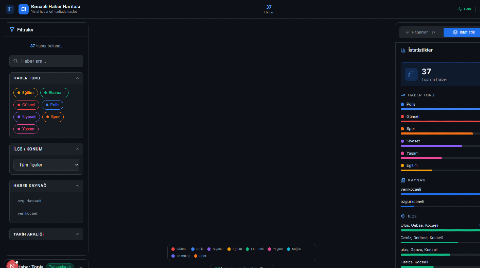
\includegraphics[width=0.55\textwidth]{image1.png}
\caption{Arayüz Görüntüsü 1 - Harita ve Filtreleme Paneli}
\label{fig:arayuz1}
\end{figure}

\begin{figure}[H]
\centering
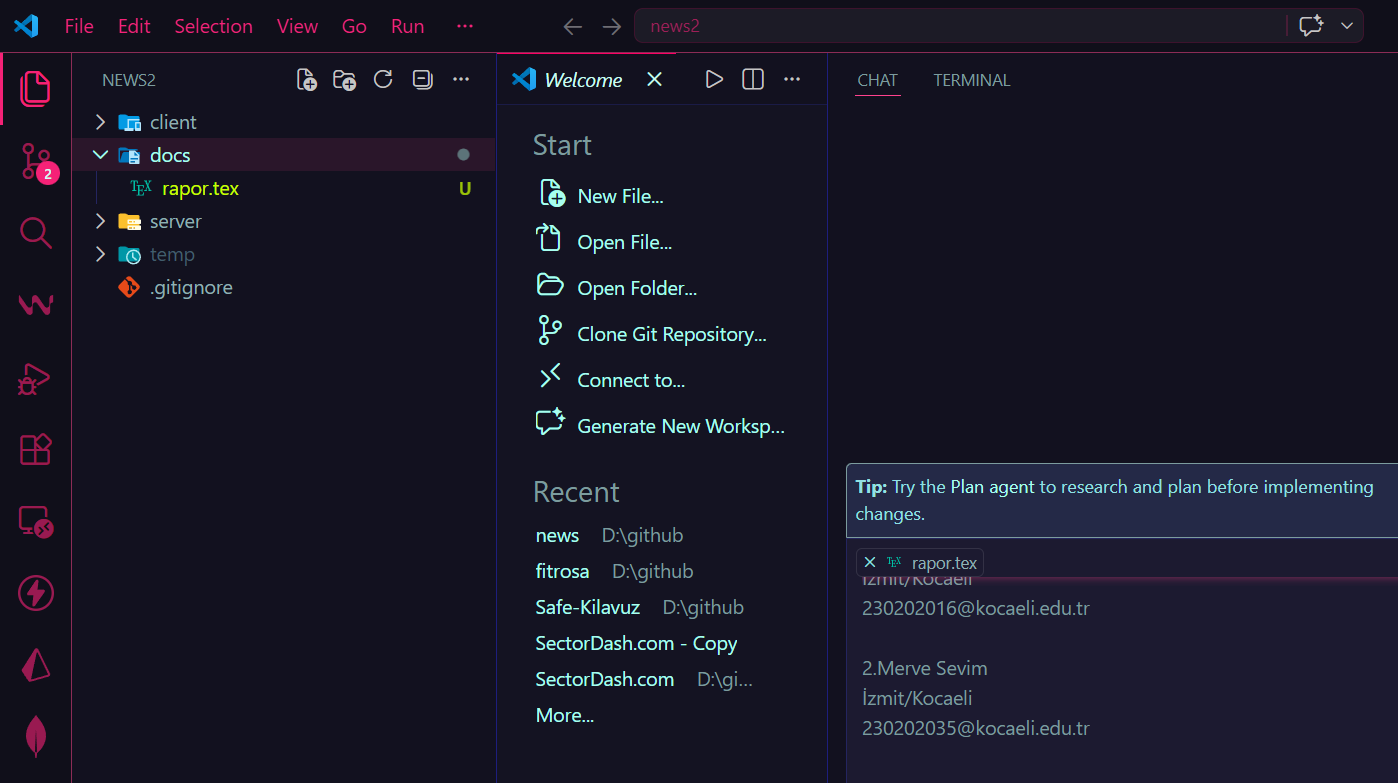
\includegraphics[width=0.55\textwidth]{image2.png}
\caption{Arayüz Görüntüsü 2 - Detaylı Haber Görünümü}
\label{fig:arayuz2}
\end{figure}

% ──────────────────────────────────────────────
\section*{Teşekkür}

Bu çalışma, Kocaeli Üniversitesi Bilgisayar Mühendisliği Bölümü bünyesinde gerçekleştirilmiştir. Değerli katkıları için danışmanlarımıza teşekkür ederiz.

% ──────────────────────────────────────────────
\begin{thebibliography}{10}

\bibitem{liu2019}
B.~Liu, \emph{Web Data Mining: Exploring Hyperlinks, Contents, and Usage Data}, 2nd~ed. Springer, 2019.

\bibitem{mitchell2018}
R.~Mitchell, \emph{Web Scraping with Python: Collecting More Data from the Modern Web}, 2nd~ed. O'Reilly Media, 2018.

\bibitem{jurafsky2024}
D.~Jurafsky and J.~H.~Martin, \emph{Speech and Language Processing}, 3rd~ed. (draft). Pearson, 2024.

\bibitem{reimers2019}
N.~Reimers and I.~Gurevych, ``Sentence-BERT: Sentence embeddings using Siamese BERT-networks,'' in \emph{Proc. EMNLP-IJCNLP}, 2019, pp.~3982--3992.

\bibitem{gao2020}
S.~Gao, J.~Janowicz, B.~Adams, and K.~Janowicz, ``A survey of geographic information extraction from text,'' \emph{ACM Computing Surveys}, vol.~53, no.~2, pp.~1--40, 2020.

\bibitem{mongodb2024}
MongoDB, Inc., ``MongoDB documentation,'' 2024. [Online]. Available: \url{https://www.mongodb.com/docs/}

\bibitem{fastapi2024}
S.~Ramírez, ``FastAPI documentation,'' 2024. [Online]. Available: \url{https://fastapi.tiangolo.com/}

\bibitem{beautifulsoup2024}
L.~Richardson, ``Beautiful Soup documentation,'' 2024. [Online]. Available: \url{https://www.crummy.com/software/BeautifulSoup/}

\bibitem{nextjs2024}
Vercel, ``Next.js documentation,'' 2024. [Online]. Available: \url{https://nextjs.org/docs}

\bibitem{googlemaps2024}
Google, ``Google Maps Platform documentation,'' 2024. [Online]. Available: \url{https://developers.google.com/maps}

\end{thebibliography}

\end{document}
